\chapter{Szczegóły implementacji}
\section{Serwer i baza danych}
Zgodnie z diagramem architektury systemu, serwer składa się z kilku modułów.
Klient ma o wiele prostszą budowę, składa się głównie z warstwy interfejsu użytkownika, logiki odpowiedzialnej za komunikację z REST API oraz obsługi JWT.
\subsection{REST API}
API jest podzielone na 2 główne foldery: \texttt{Controllers} oraz \texttt{Requests}. 
Folder \texttt{Controllers} zawiera kontrolery obsługujące żądania HTTP, natomiast \texttt{Requests} zawiera klasy reprezentujące żądania wysyłane przez klienta do API.
Poza nimi znajdują się również foldery \texttt{Extensions} oraz \texttt{Utils}, które zawierają odpowiednio rozszerzenia dla rejestracji punktów końcowych oraz klasę \texttt{BearerSecuritySchemeTransformer}.
Ma ona na celu dodanie obsługi schematu bezpieczeństwa posiadacza (ang.~\emph{Bearer security scheme}) do dokumentacji API. 
Pozwala to na dodanie w łatwy sposób tokenu uzyskanego po zalogowaniu do nagłówków żądań wysyłanych do API.
Opisaną strukturę projektu API przedstawiono na listingu \ref{list:apiStructure}.
\begin{lstlisting}[label=list:apiStructure,caption=Struktura projektu API,style=folderview]
Eider-Rider.Api
|-- Controllers
|   |-- CarController.cs
|   |-- ReservationController.cs
|   |-- RouteController.cs
|   \-- UserController.cs
|-- Extensions
|   \-- EndpointRouteBuilderExtensions.cs
|-- Program.cs
|-- Requests
|   |-- Cars
|   |   |-- CreateCarRequest.cs
|   |   \-- UpdateCarRequest.cs
|   |-- Reservations
|   |   |-- CreateReservationRequest.cs
|   |   \-- UpdateReservationRequest.cs
|   |-- Routes
|   |   |-- CreateRouteRequest.cs
|   |   \-- MatchRouteRequest.cs
|   \-- Users
|       |-- LoginRequest.cs
|       |-- RefreshTokenRequest.cs
|       \-- RegisterRequest.cs
\-- Utils
    \-- BearerSecuritySchemeTransformer.cs
\end{lstlisting}
Samo API zostało zaprojektowane w podejściu minimalnym \cite{MS_APIS}. 
Jest to uproszczone, wysokowydajne podejście do tworzenia interfejsów API z minimalnym kodem i konfiguracją.
W każdym kontrolerze znajduje się metoda rejestrująca punkty końcowe obsługiwane przez dany kontroler, w której definiowane są również role użytkowników mające dostęp do poszczególnych punktów końcowych.
Przykład takiej metody pokazano na listingu \ref{list:mapEndpointsExample}.
\begin{lstlisting}[label=list:mapEndpointsExample,caption=Przykład rejestracji punktów końcowych,style=sharpcstyle]
public static class ReservationController
{
    public static IEndpointRouteBuilder MapReservations(this IEndpointRouteBuilder endpoints)
    {
        var group = endpoints.MapGroup("/reservations");
        
        group.WithTags("Reservations");

        group.MapGet("/get/{routeId:Guid}", GetReservationByRouteIdAsync)
            .RequireAuthorization(PolicyNames.Driver);
        [...]

        group.MapPost("/create", CreateReservationAsync)
            .RequireAuthorization(PolicyNames.Passenger);
        [...]
        
        return endpoints;
    }
    [...]
\end{lstlisting}
\begin{table}[htb]
\small
\centering
\caption{Punkty końcowe kontrolera \texttt{CarController}}
\label{tab:endpoints-car}
\begin{tabularx}{\linewidth}{|c|X|X|} \hline
Typ & Ścieżka & Opis \\ \hline\hline
\texttt{POST} & \texttt{/car/create} & Tworzy samochód kierowcy. \\ \hline
\texttt{PUT} & \texttt{/car/update} & Aktualizuje dane samochodu kierowcy. \\ \hline
\texttt{GET} & \texttt{/car/} & Pobiera dane samochodu kierowcy. \\ \hline
\end{tabularx}
\end{table}

\begin{table}[htb]
\small
\centering
\caption{Punkty końcowe kontrolera \texttt{ReservationController}}
\label{tab:endpoints-reservation}
\begin{tabularx}{\linewidth}{|c|X|X|} \hline
Typ & Ścieżka & Opis \\ \hline\hline
\texttt{GET} & \texttt{/reservations/get/\{Guid\}} & Pobiera rezerwację dla wskazanej trasy. \\ \hline
\texttt{GET} & \texttt{/reservations/mine} & Pobiera rezerwacje pasażera. \\ \hline
\texttt{POST} & \texttt{/reservations/create} & Tworzy rezerwację. \\ \hline
\texttt{POST} & \texttt{/reservations/update} & Aktualizuje rezerwację. \\ \hline
\texttt{DELETE} & \texttt{/reservations/delete/\{Guid\}} & Usuwa wskazaną rezerwację. \\ \hline
\end{tabularx}
\end{table}

\begin{table}[htb]
\small
\centering
\caption{Punkty końcowe kontrolera \texttt{RouteController}}
\label{tab:endpoints-route}
\begin{tabularx}{\linewidth}{|c|X|X|} \hline
Typ & Ścieżka & Opis \\ \hline\hline
\texttt{POST} & \texttt{/routes/create} & Tworzy trasę. \\ \hline
\texttt{POST} & \texttt{/routes/match} & Wyszukuje pasującą trasę. \\ \hline
\texttt{GET} & \texttt{/routes/} & Pobiera trasy kierowcy. \\ \hline
\texttt{GET} & \texttt{/routes/path/\{Guid\}} & Pobiera przebieg trasy. \\ \hline
\texttt{DELETE} & \texttt{/routes/cancel/\{Guid\}} & Anuluje wskazaną trasę. \\ \hline
\end{tabularx}
\end{table}

\begin{table}[htb]
\small
\centering
\caption{Punkty końcowe kontrolera \texttt{UserController}}
\label{tab:endpoints-user}
\begin{tabularx}{\linewidth}{|c|X|X|} \hline
Typ & Ścieżka & Opis \\ \hline\hline
\texttt{POST} & \texttt{/users/login} & Loguje użytkownika. \\ \hline
\texttt{POST} & \texttt{/users/register/user} & Rejestruje pasażera. \\ \hline
\texttt{POST} & \texttt{/users/register/driver} & Rejestruje kierowcę. \\ \hline
\texttt{POST} & \texttt{/users/token/refresh} & Odświeża token dostępu. \\ \hline
\texttt{GET} & \texttt{/users/} & Pobiera dane użytkownika. \\ \hline
\end{tabularx}
\end{table}

\subsection{Warstwa logiki biznesowej}
\subsection{Warstwa uwierzytelniania i autoryzacji}
\subsection{Warstwa dostępu do bazy danych}
\begin{figure}[h]
	\centering
	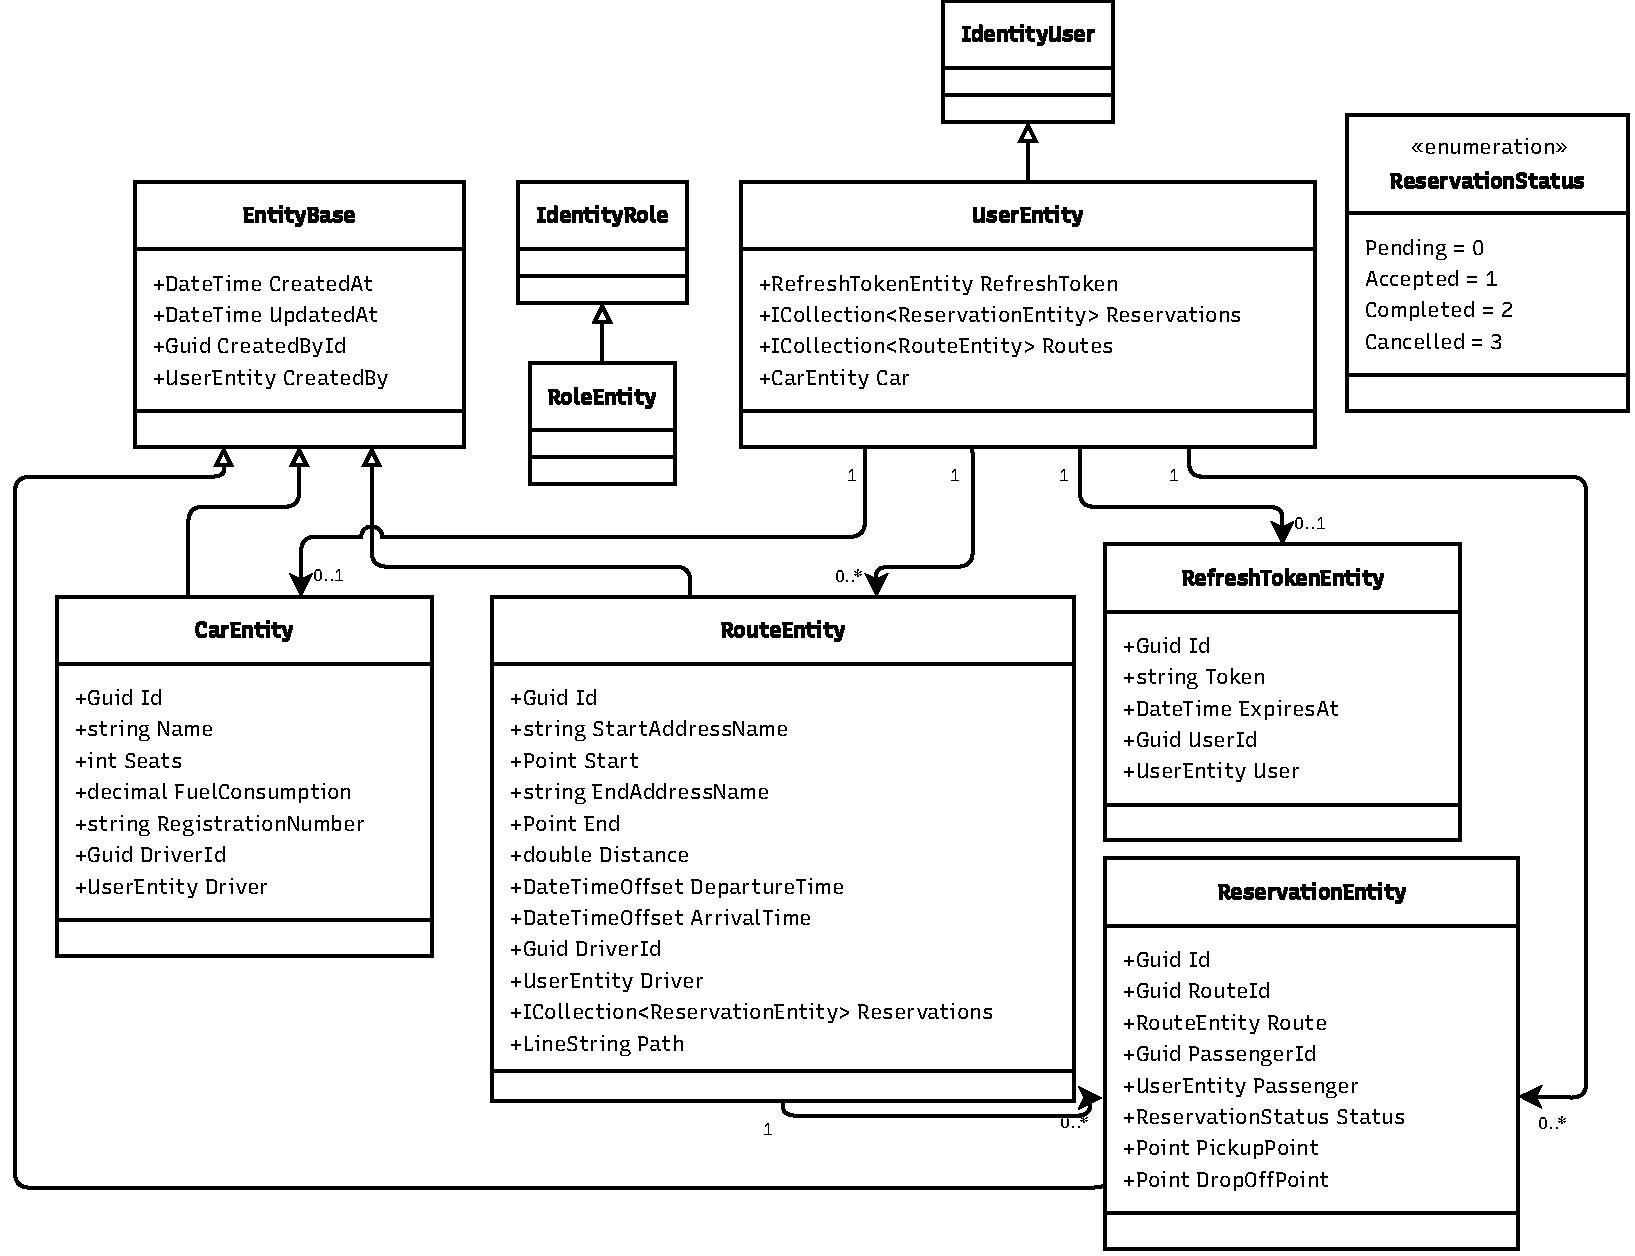
\includegraphics[width=0.9\linewidth]{rys04/CLASS_ER-v2.drawio.pdf}
	\caption{Diagram relacji klas encji}
	\label{fig:entity-class-diagram}
\end{figure}
\section{Aplikacja internetowa}
\subsection{Struktura aplikacji}
\subsection{Interfejs użytkownika}
\subsection{Integracja z REST API}